% lint-skip: 未完成ステータス（figure/table caption 未対応，人手チェック時に解消予定）
\documentclass[../../main.tex]{subfiles}
\begin{document}

\begin{flushright}
  \footnotesize\textit{【自動文字起こし・要確認】}
\end{flushright}

\noindent
{\bf [解答]} $f_q(x) = x^4 - 6p^2 x^2 - 8q^3 x$ とおく. ($p > 0, q \ge 0$)

$f_q'(x) = 4x^3 - 12p^2 x - 8q^3$ だから, $q=0$ の時, 下表を得る

\begin{center}
  \begin{table}[htb]
    \centering
    \begin{tabular}{c|c|c|c|c|c|c|c}
      $x$ & $\dots$ & $-\sqrt{3}p$ & $\dots$ & $0$ & $\dots$ & $\sqrt{3}p$ & $\dots$ \\ \hline
      $f'$ & $-$ & $0$ & $+$ & $0$ & $-$ & $0$ & $+$ \\ \hline
      $f$ & $\searrow$ & & $\nearrow$ & & $\searrow$ & & $\nearrow$
    \end{tabular}
  \end{table}
\end{center}

\noindent
従って, $A$ の $x$ 座標は $-\sqrt{3}p \; (\equiv x_0)$ である. 又, $f_q''(x) = 12(x^2 - p^2)$ から下表を得る

\begin{center}
  \begin{table}[htb]
    \centering
    \begin{tabular}{c|c|c|c|c|c}
      $x$ & $\dots$ & $-p$ & $\dots$ & $p$ & $\dots$ \\ \hline
      $f''$ & $+$ & $0$ & $-$ & $0$ & $+$ \\ \hline
      $f'$ & $\nearrow$ & 8($p^3-q^3$) & $\searrow$ & 負 & $\nearrow$
    \end{tabular}
  \end{table}
\end{center}

\noindent
従って $q$ の値により下表をえる

\bigskip
\noindent
$1^\circ$ $p > q$ の時

$f_q'(-p) > 0$ から, $f_q'(x) = 0$ となる $x$ が 3つある ($\alpha < \beta < \gamma$ とする)

\begin{center}
  \begin{table}[htb]
    \centering
    \begin{tabular}{c|c|c|c|c|c|c|c}
      $x$ & $\dots$ & $\alpha$ & $\dots$ & $\beta$ & $\dots$ & $\gamma$ & $\dots$ \\ \hline
      $f'$ & $-$ & $0$ & $+$ & $0$ & $-$ & $0$ & $+$ \\ \hline
      $f$ & $\searrow$ & & $\nearrow$ & & $\searrow$ & & $\nearrow$
    \end{tabular}
  \end{table}
\end{center}

\noindent
この時 $A$ が右のくぼみに落ちるのは, $\beta \le -\sqrt{3}p \le \gamma$ の時である. $\quad \cdots \text{①}$

\noindent
しかし, 本から $-p < \beta$ であり, 又 $p > 0$ から $-\sqrt{3}p < -p$ だから ①がみたされることはなく, 矛盾.

\bigskip
\noindent
$2^\circ$ $p \le q$ の時

$f_q'(-p) \le 0$ から, $f_q'(x) = 0$ となる $x$ が唯一存在する ($\alpha$ とする)

\begin{center}
  \begin{table}[htb]
    \centering
    \begin{tabular}{c|c|c|c}
      $x$ & $\dots$ & $\alpha$ & $\dots$ \\ \hline
      $f'$ & $-$ & $0$ & $+$ \\ \hline
      $f$ & $\searrow$ & & $\nearrow$
    \end{tabular}
  \end{table}
\end{center}

\noindent
よって, $A$ が右のくぼみに落ちるのは $-\sqrt{3}p \le \alpha$ つまり $f_q'(-\sqrt{3}p) \le 0$ の時,
\[
  f_q'(-\sqrt{3}p) = -8q^3 \le 0 \quad \therefore q \ge 0
\]
したがって, $0 < p$ から $p \le q$ の時, $A$ が右のくぼみにおちる.

\noindent
以上 $1^\circ, 2^\circ$ から求める $\min q = p$ である.

\begin{figure}[htb]
  \centering
  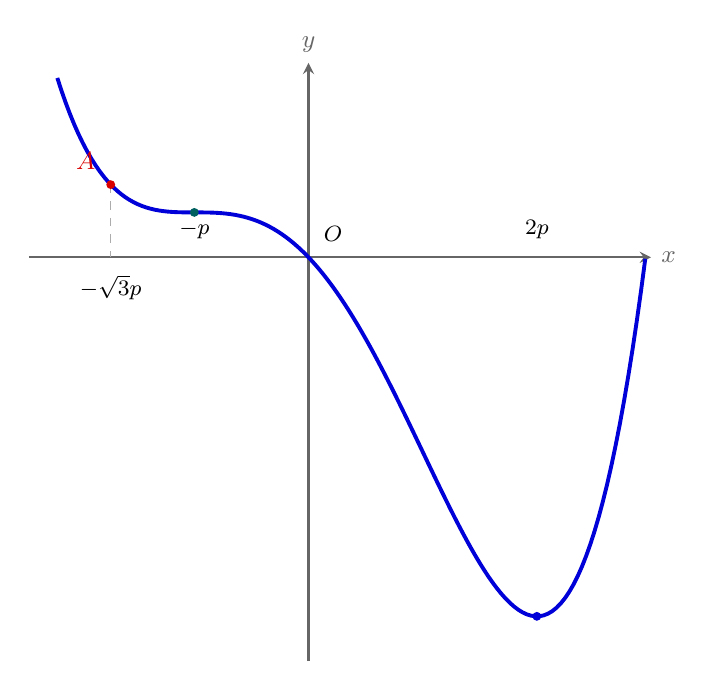
\begin{tikzpicture}[x=1.45cm, y=0.19cm, >=stealth,
    every node/.style={font=\small}]
    % Normalize p=q=1; f(x)=x^4-6x^2-8x, with f'=4(x+1)^2(x-2).
    \coordinate (A) at ({-sqrt(3)},{9-18+8*sqrt(3)});
    \coordinate (I) at (-1,3);
    \coordinate (Min) at (2,-24);
    \draw[->, thick, gray!80!black] (-2.45,0) -- (3.0,0) node[right] {$x$};
    \draw[->, thick, gray!80!black] (0,-27) -- (0,13) node[above] {$y$};
    \draw[dashed, gray!65] (A) -- ({-sqrt(3)},0);
    \draw[line width=1.4pt, blue!85!black, domain=-2.2:2.95, samples=140]
    plot (\x,{\x*\x*\x*\x-6*\x*\x-8*\x});
    \fill[red!85!black] (A) circle (1.6pt);
    \fill[teal!75!black] (I) circle (1.6pt);
    \fill[blue!85!black] (Min) circle (1.6pt);
    \node[above left=2pt, red!85!black] at (A) {$A$};
    \node[below=3pt, font=\footnotesize] at ({-sqrt(3)},0) {$-\sqrt3p$};
    \node[above=3pt, font=\footnotesize] at (-1,0) {$-p$};
    \node[above=3pt, font=\footnotesize] at (2,0) {$2p$};
    \node[above right=2pt, font=\footnotesize] at (0,0) {$O$};
  \end{tikzpicture}
  \caption{$q=p$ の境界で，$x=-p$ に水平な変曲点が現れる}
\end{figure}
\noindent
$\left[\text{この時, } f'(x) = 4(x^3 - 3p^2 x - 2p^3) = 4(x+p)^2 (x-2p) \text{ となり,}\right]$ $\Rightarrow$ 予想通り!

\newpage

\end{document}
